\documentclass[tikz,border=10pt]{standalone}
\usepackage{tikz}
\usepackage{amsmath}

\begin{document}
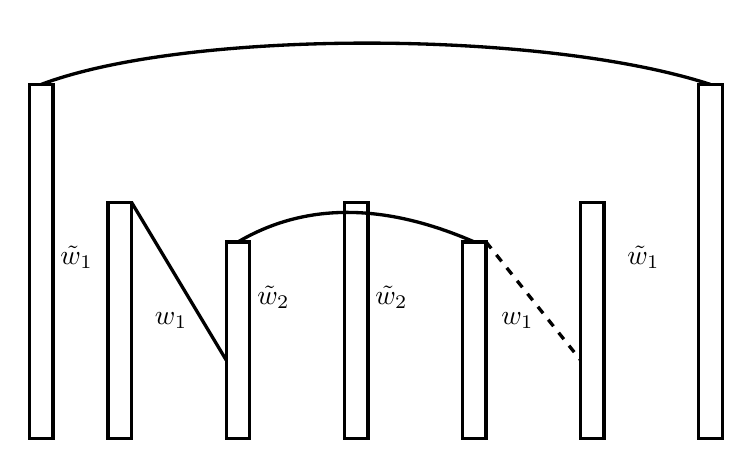
\begin{tikzpicture}[scale=1, line width=1.2pt]

% Outer left column
\draw (0,0) rectangle (0.3,4.5);

% Inner left column  
\draw (1,0) rectangle (1.3,3);

% Left middle column
\draw (2.5,0) rectangle (2.8,2.5);

% Center column
\draw (4,0) rectangle (4.3,3);

% Right middle column
\draw (5.5,0) rectangle (5.8,2.5);

% Inner right column
\draw (7,0) rectangle (7.3,3);

% Outer right column
\draw (8.5,0) rectangle (8.8,4.5);

% Top arch connecting outer columns
\draw (0.15,4.5) .. controls (2,5.2) and (6.5,5.2) .. (8.65,4.5);

% Inner arch
\draw (2.65,2.5) .. controls (3.5,3) and (4.5,3) .. (5.65,2.5);

% Diagonal solid line
\draw (1.3,3) -- (2.5,1);

% Diagonal dashed line  
\draw[dashed] (5.8,2.5) -- (7,1);

% Labels
\node at (0.6,2.3) {$\tilde{w}_1$};
\node at (1.8,1.5) {$w_1$};
\node at (3.1,1.8) {$\tilde{w}_2$};
\node at (4.6,1.8) {$\tilde{w}_2$};
\node at (6.2,1.5) {$w_1$};
\node at (7.8,2.3) {$\tilde{w}_1$};

\end{tikzpicture}
\end{document}